\section{Data Investigation}

For the data investigation task, I took 3 files and ran 6 different configurations on each one of them. The tables below contain the results of 3 runs against each configuration.

\subsection{Results for inst-0.tsp}
For \textit{inst-0.tsp} file the below results have been collected with varying attributes.

\begin{itemize}
  \item Population size of 300
  \item Mutation rate of 0.1
  \item Max iterations of 300
\end{itemize}

\begin{table}[H]
\resizebox{\textwidth}{!}{%
\begin{tabular}{lllllll}
\rowcolor[HTML]{ECF4FF} 
Configuration                               & 1                & 2                & 3                & 4                & 5                & 6                \\
\cellcolor[HTML]{ECF4FF}Time (s)            & 29               & 45               & 31               & 59               & 60               & 32               \\
\cellcolor[HTML]{ECF4FF}Initial Best        & 22565794.0154538 & 22760929.3954624 & 23149493.7224535 & 23020079.1572776 & 22804748.2104552 & 22980219.8748152 \\
\cellcolor[HTML]{ECF4FF}Best                & 21783889.1480634 & 21083853.8657483 & 21731665.4546834 & 21354797.1361259 & 21599161.1651287 & 22374565.4048446 \\
\cellcolor[HTML]{ECF4FF}Improvement (\%)    & 3.47             & 7.37             & 6.12             & 7.23             & 5.29             & 2.64             \\
\cellcolor[HTML]{ECF4FF}                    &                  &                  &                  &                  &                  &                  \\
\cellcolor[HTML]{ECF4FF}Time (s)            & 29               & 45               & 30               & 58               & 60               & 32               \\
\cellcolor[HTML]{ECF4FF}Initial Best        & 22807873.8594888 & 22709548.6661797 & 22908989.5897279 & 21948033.7019009 & 22613853.9197897 & 23001623.9066584 \\
\cellcolor[HTML]{ECF4FF}Best                & 21611574.4431279 & 21125521.1226399 & 21433219.7879355 & 21463300.5883081 & 21426354.9669659 & 23001623.9066584 \\
\cellcolor[HTML]{ECF4FF}Improvement (\%)    & 5.25             & 6.98             & 6.44             & 2.21             & 5.25             & 0.00             \\
\cellcolor[HTML]{ECF4FF}                    &                  &                  &                  &                  &                  &                  \\
\cellcolor[HTML]{ECF4FF}Time (s)            & 29               & 45               & 31               & 59               & 60               & 34               \\
\cellcolor[HTML]{ECF4FF}Initial Best        & 22913634.9815796 & 22593038.9233456 & 22902355.9017428 & 22740659.8220616 & 22791673.5572732 & 22409526.3564714 \\
\cellcolor[HTML]{ECF4FF}Best                & 21121033.2077978 & 21593746.3381396 & 21684282.0059868 & 21431688.3535831 & 21542513.8985687 & 22409526.3564714 \\
\cellcolor[HTML]{ECF4FF}Improvement(\%)     & 7.82             & 4.42             & 5.32             & 5.76             & 5.48             & 0.00             \\
\rowcolor[HTML]{CBCEFB} 
\cellcolor[HTML]{DAE8FC}Average Run Time    & 29.00            & 45.00            & 30.67            & 58.67            & 60.00            & 32.67            \\
\rowcolor[HTML]{CBCEFB} 
\cellcolor[HTML]{DAE8FC}Average Best        & 21505498.9329964 & 21267707.1088426 & 21616389.0828686 & 21416595.359339  & 21522676.6768878 & 22595238.5559915 \\
\rowcolor[HTML]{CBCEFB} 
\cellcolor[HTML]{DAE8FC}Average Improvement & 5.51             & 6.26             & 5.96             & 5.07             & 5.34             & 0.88             \\
\rowcolor[HTML]{CBCEFB} 
\cellcolor[HTML]{DAE8FC}Median              & 21611574.4431279 & 21125521.1226399 & 21684282.0059868 & 21431688.3535831 & 21542513.8985687 & 22409526.3564714
\end{tabular}%
}
\end{table}

\begin{itemize}
  \item Population size of 400
  \item Mutation rate of 0.1
  \item Max iterations of 300
\end{itemize}

\begin{table}[H]
\resizebox{\textwidth}{!}{%
\begin{tabular}{lllllll}
\rowcolor[HTML]{ECF4FF} 
Configuration                               & 1                & 2                & 3                & 4                & 5                & 6                 \\
\cellcolor[HTML]{ECF4FF}Time (s)            & 118              & 61               & 144              & 86               & 88               & 180               \\
\cellcolor[HTML]{ECF4FF}Initial Best        & 22683710.5632501 & 22197330.297332  & 22820351.7158666 & 22494359.5260535 & 22798342.5798216 & 22419232.7900901  \\
\cellcolor[HTML]{ECF4FF}Best                & 21355880.5073546 & 21268340.707675  & 21688524.8733755 & 21417045.1661967 & 21175882.9558971 & 22419232.7900901  \\
\cellcolor[HTML]{ECF4FF}Improvement (\%)    & 5.85             & 4.19             & 4.96             & 4.79             & 7.12             & 0.00              \\
\cellcolor[HTML]{ECF4FF}                    &                  &                  &                  &                  &                  &                   \\
\cellcolor[HTML]{ECF4FF}Time (s)            & 119              & 60               & 143              & 86               & 88               & 179               \\
\cellcolor[HTML]{ECF4FF}Initial Best        & 22444355.736871  & 22716490.7518481 & 22993608.5218155 & 22761725.5456394 & 22668885.7139625 & 22915080.7829117  \\
\cellcolor[HTML]{ECF4FF}Best                & 21388788.9753153 & 21448274.5766078 & 21123235.2480732 & 21327764.2612524 & 21489316.3328765 & 22904265.8504637  \\
\cellcolor[HTML]{ECF4FF}Improvement (\%)    & 4.70             & 5.58             & 8.13             & 6.30             & 5.20             & 0.05              \\
\cellcolor[HTML]{ECF4FF}                    &                  &                  &                  &                  &                  &                   \\
\cellcolor[HTML]{ECF4FF}Time (s)            & 118              & 61               & 145              & 87               & 88               & 180               \\
\cellcolor[HTML]{ECF4FF}Initial Best        & 22723717.1860885 & 22655164.0372629 & 22398910.2865146 & 22403573.3062295 & 22806465.12461   & 22723486.4916315  \\
\cellcolor[HTML]{ECF4FF}Best                & 21497987.3249621 & 21404852.1592652 & 21466620.8955464 & 21354803.2278426 & 21330955.7101958 & 22723486.4916315  \\
\cellcolor[HTML]{ECF4FF}Improvement(\%)     & 5.39             & 5.52             & 4.16             & 4.68             & 6.47             & 0.00              \\
\rowcolor[HTML]{CBCEFB} 
\cellcolor[HTML]{DAE8FC}Average Run Time    & 118.33           & 60.67            & 144.00           & 86.33            & 88.00            & 179.67            \\
\rowcolor[HTML]{CBCEFB} 
\cellcolor[HTML]{DAE8FC}Average Best        & 21414218.9358773 & 21373822.4811827 & 21426127.005665  & 21366537.5517639 & 21332051.6663231 & 22682328.3773951  \\
\rowcolor[HTML]{CBCEFB} 
\cellcolor[HTML]{DAE8FC}Average Improvement & 5.32             & 5.10             & 5.75             & 5.26             & 6.26             & 0.02              \\
\rowcolor[HTML]{CBCEFB} 
\cellcolor[HTML]{DAE8FC}Median              & 5.85367218556702 & 5.58279968985581 & 8.13431816049124 & 6.29987951270115 & 7.11656831299882 & 0.047195698546543
\end{tabular}%
}
\end{table}

\begin{itemize}
  \item Population size of 100
  \item Mutation rate of 0.1
  \item Max iterations of 300
\end{itemize}

\begin{table}[H]
\resizebox{\textwidth}{!}{%
\begin{tabular}{lllllll}
\rowcolor[HTML]{ECF4FF} 
Configuration                               & 1                & 2                & 3                & 4                & 5                & 6                \\
\cellcolor[HTML]{ECF4FF}Time (s)            & 29               & 15               & 31               & 16               & 16               & 33               \\
\cellcolor[HTML]{ECF4FF}Initial Best        & 22894685.6885232 & 22158299.6131183 & 22659393.9342978 & 22495269.1871355 & 22367415.1141798 & 22868149.2155585 \\
\cellcolor[HTML]{ECF4FF}Best                & 21907599.6526283 & 21794369.4246789 & 21550838.8530944 & 21524637.1076923 & 21683890.6088459 & 22854002.3292278 \\
\cellcolor[HTML]{ECF4FF}Improvement (\%)    & 4.31             & 1.64             & 4.89             & 4.31             & 3.06             & 0.06             \\
\cellcolor[HTML]{ECF4FF}                    &                  &                  &                  &                  &                  &                  \\
\cellcolor[HTML]{ECF4FF}Time (s)            & 29               & 15               & 31               & 16               & 16               & 32               \\
\cellcolor[HTML]{ECF4FF}Initial Best        & 22916347.1773741 & 22717004.8326221 & 23078816.5088211 & 22970036.7420101 & 23234065.5509564 & 22529636.6011284 \\
\cellcolor[HTML]{ECF4FF}Best                & 21657097.5682132 & 21519784.6919748 & 21816883.5840052 & 21157988.8736445 & 21771619.3496972 & 22529636.6011284 \\
\cellcolor[HTML]{ECF4FF}Improvement (\%)    & 5.49             & 5.27             & 5.47             & 7.89             & 6.29             & 0.00             \\
\cellcolor[HTML]{ECF4FF}                    &                  &                  &                  &                  &                  &                  \\
\cellcolor[HTML]{ECF4FF}Time (s)            & 29               & 15               & 31               & 16               & 16               & 33               \\
\cellcolor[HTML]{ECF4FF}Initial Best        & 22522914.2521871 & 23061374.1695362 & 22977516.670363  & 23037115.7226756 & 22800099.7446576 & 22912816.2576871 \\
\cellcolor[HTML]{ECF4FF}Best                & 21727154.6212607 & 21640478.838916  & 21816883.5840052 & 21772738.8169103 & 21574381.1935916 & 22912816.2576871 \\
\cellcolor[HTML]{ECF4FF}Improvement(\%)     & 3.53             & 6.16             & 5.05             & 5.49             & 5.38             & 0.00             \\
\rowcolor[HTML]{CBCEFB} 
\cellcolor[HTML]{DAE8FC}Average Run Time    & 29.00            & 15.00            & 31.00            & 16.00            & 16.00            & 32.67            \\
\rowcolor[HTML]{CBCEFB} 
\cellcolor[HTML]{DAE8FC}Average Best        & 21763950.6140341 & 21651544.3185232 & 21728202.0070349 & 21485121.5994157 & 21676630.3840449 & 22765485.0626811 \\
\rowcolor[HTML]{CBCEFB} 
\cellcolor[HTML]{DAE8FC}Average Improvement & 4.45             & 4.36             & 5.14             & 5.90             & 4.91             & 0.02             \\
\rowcolor[HTML]{CBCEFB} 
\cellcolor[HTML]{DAE8FC}Median              & 21692126.0947369 & 21580131.7654454 & 21683861.2185498 & 21341312.9906684 & 21629135.9012187 & 22691819.4651781
\end{tabular}%
}
\end{table}

\begin{itemize}
  \item Population size of 300
  \item Mutation rate of 0.5
  \item Max iterations of 300
\end{itemize}

\begin{table}[H]
\resizebox{\textwidth}{!}{%
\begin{tabular}{lllllll}
\rowcolor[HTML]{ECF4FF} 
Configuration                               & 1                & 2                & 3                & 4                & 5                & 6                \\
\cellcolor[HTML]{ECF4FF}Time (s)            & 84               & 40               & 99               & 54               & 55               & 116              \\
\cellcolor[HTML]{ECF4FF}Initial Best        & 22350512.3258509 & 22458508.0509341 & 22609369.5518849 & 22710633.2690212 & 22763632.842259  & 22516010.339516  \\
\cellcolor[HTML]{ECF4FF}Best                & 21421006.7074661 & 21027147.6550745 & 21913374.2125168 & 21623162.8936265 & 21350014.1858509 & 22016367.2624037 \\
\cellcolor[HTML]{ECF4FF}Improvement (\%)    & 4.16             & 6.37             & 3.08             & 4.79             & 6.21             & 2.22             \\
\cellcolor[HTML]{ECF4FF}                    &                  &                  &                  &                  &                  &                  \\
\cellcolor[HTML]{ECF4FF}Time (s)            & 85               & 40               & 99               & 54               & 55               & 118              \\
\cellcolor[HTML]{ECF4FF}Initial Best        & 21872515.3946241 & 22558305.9204958 & 22359511.4462861 & 22589455.5781608 & 22463689.5921854 & 22209517.698716  \\
\cellcolor[HTML]{ECF4FF}Best                & 21270011.2739576 & 21849205.0738998 & 21215230.9365659 & 21481974.8394946 & 21511765.5770896 & 22209517.698716  \\
\cellcolor[HTML]{ECF4FF}Improvement (\%)    & 2.75             & 3.14             & 5.12             & 4.90             & 4.24             & 0.00             \\
\cellcolor[HTML]{ECF4FF}                    &                  &                  &                  &                  &                  &                  \\
\cellcolor[HTML]{ECF4FF}Time (s)            & 1                & 2                & 3                & 4                & 5                & 6                \\
\cellcolor[HTML]{ECF4FF}Initial Best        & 86               & 40               & 99               & 55               & 55               & 117              \\
\cellcolor[HTML]{ECF4FF}Best                & 22557787.5980914 & 22712365.5366604 & 22897573.0061196 & 22415996.4029482 & 22482769.6884155 & 22527996.0494822 \\
\cellcolor[HTML]{ECF4FF}Improvement(\%)     & 21308050.0556079 & 21485939.3722828 & 21523116.5156892 & 21232228.0836397 & 21283335.779742  & 22527996.0494822 \\
\rowcolor[HTML]{CBCEFB} 
\cellcolor[HTML]{DAE8FC}Average Run Time    & 85.00            & 40.00            & 99.00            & 54.33            & 55.00            & 117.00           \\
\rowcolor[HTML]{CBCEFB} 
\cellcolor[HTML]{DAE8FC}Average Best        & 21333022.6790105 & 21454097.3670857 & 21550573.8882573 & 21445788.6055869 & 21381705.1808942 & 22251293.6702006 \\
\rowcolor[HTML]{CBCEFB} 
\cellcolor[HTML]{DAE8FC}Average Improvement & 4.15             & 4.97             & 4.73             & 4.99             & 5.26             & 0.74             \\
\rowcolor[HTML]{CBCEFB} 
\cellcolor[HTML]{DAE8FC}Median              & 21308050.0556079 & 21485939.3722828 & 21523116.5156892 & 21481974.8394946 & 21350014.1858509 & 22209517.698716 
\end{tabular}%
}
\end{table}

\begin{figure}[H]
\vspace{-5pt}
\centering
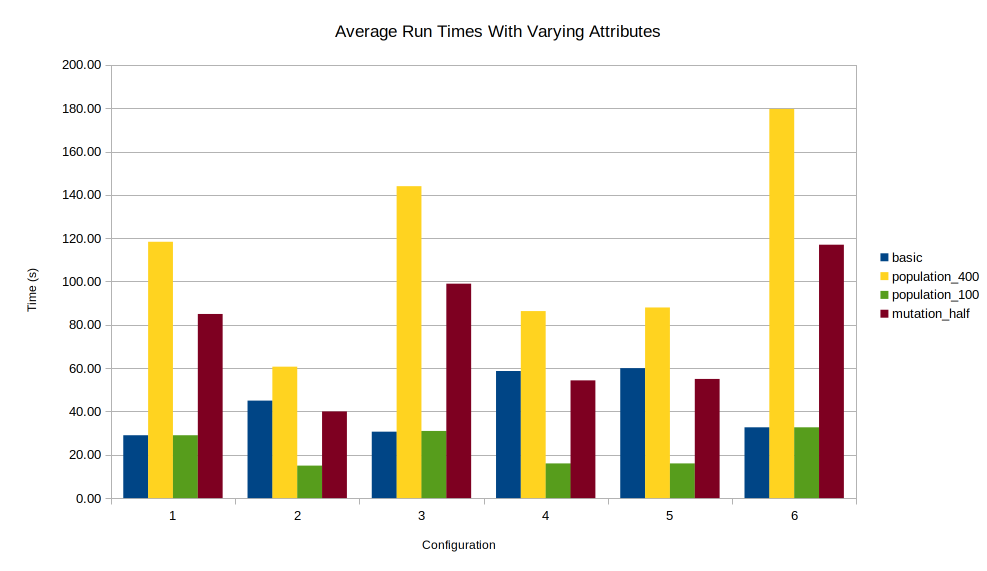
\includegraphics[width=1.0\textwidth]{images/inst-0-run-time.png}
\caption{\label{fig:inst-0-run-time}Average run time for inst-0.tsp file versus required configurations}
\end{figure}

The average run times are shown in \ref{fig:inst-0-run-time} show that configuration 6 with a population size of 400 drastically increases the runtime. This is not surprising as there is a lot more data to process.
Increasing the mutation rate to 0.9 also affects the runtime as can be seen from \ref{fig:inst-0-run-time} depicted in the \textit{mutation half} bar. Again this is not surprising as we will be mutating more often then we would have been with a mutation rate of 0.1 resulting in more processing.

\begin{figure}[H]
\vspace{-5pt}
\centering
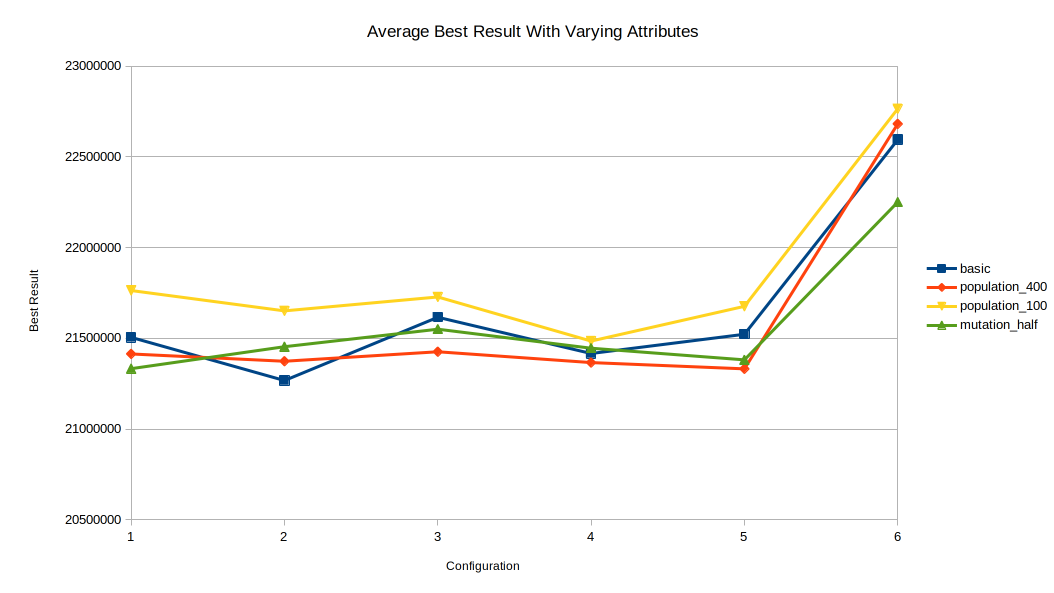
\includegraphics[width=1.0\textwidth]{images/inst-0-average-best.png}
\caption{\label{fig:inst-0-average-best}Average best result for inst-0.tsp file versus required configurations}
\end{figure}

The best average results are shown in \ref{fig:inst-0-average-best}. Configuration 2 performed well here without varying population size or mutation rate. However, this does seem to vary wildly between configurations. Increasing the population seems to be uniform across each configuration excluding configuration 6. Interestingly decreasing the population to 100 seems to have reported the worst results across each configuration.

Configuration 6 which includes the best and second best selection method seems to perform terribly across each of the test files, and very rarely did it find results that were better than the initial best result, my best guess as to why this is, is that the population is not diverse enough as we are always selecting the best and second best candidates.

\begin{figure}[H]
\vspace{-5pt}
\centering
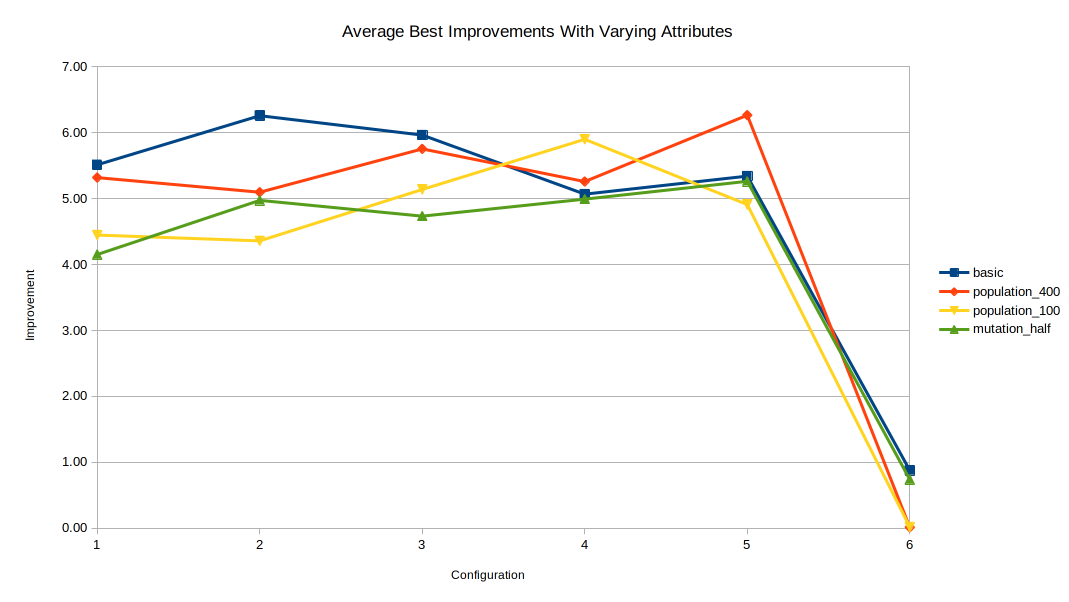
\includegraphics[width=1.0\textwidth]{images/inst-0-best-improvements.png}
\caption{\label{fig:inst-0-best-improvements}Average best improvement for inst-0.tsp file versus required configurations}
\end{figure}

In figure \ref{fig:inst-0-best-improvements} I have charted the results of the best improvement over the initial best result. 

\begin{equation}\label{eq:inst-0-best-improvement}
bestImprovement = ((initialBest - best) / initialBest) * 100
\end{equation}

As mentioned previously configuration 6 can be seen here to not be improving much at all over the initial best result. Increasing the population to 400 has been shown to be the best improvement over the initial best for configuration 5. The basic configuration without any variation seems to perform reasonably well across each configuration with the exception of configuration 6.

\subsection{Results for inst-13.tsp}

For \textit{inst-13.tsp} file, the below results have been collected with varying attributes.

\begin{itemize}
  \item Population size of 300
  \item Mutation rate of 0.1
  \item Max iterations of 300
\end{itemize}

\begin{table}[H]
\resizebox{\textwidth}{!}{%
\begin{tabular}{lllllll}
\rowcolor[HTML]{ECF4FF} 
Configuration                               & 1                & 2                & 3                & 4                & 5                & 6                \\
\cellcolor[HTML]{ECF4FF}Time (s)            & 82               & 90               & 83               & 103              & 105              & 85               \\
\cellcolor[HTML]{ECF4FF}Initial Best        & 118516136.254406 & 112214169.294359 & 116682071.408645 & 109669261.126843 & 115115757.298036 & 117623409.848751 \\
\cellcolor[HTML]{ECF4FF}Best                & 107413491.606079 & 107342105.867232 & 105083603.912513 & 102238647.451201 & 106379935.984749 & 110379760.860923 \\
\cellcolor[HTML]{ECF4FF}Improvement (\%)    & 5.32             & 2.99             & 8.36             & 6.90             & 0.00             & 0.00             \\
\cellcolor[HTML]{ECF4FF}                    &                  &                  &                  &                  &                  &                  \\
\cellcolor[HTML]{ECF4FF}Time (s)            & 81               & 90               & 83               & 104              & 104              & 85               \\
\cellcolor[HTML]{ECF4FF}Initial Best        & 118060831.266344 & 113006740.484604 & 117304856.968518 & 112684925.445101 & 113641378.488124 & 113622876.247535 \\
\cellcolor[HTML]{ECF4FF}Best                & 109377223.36932  & 107785756.571118 & 105898711.638493 & 103911944.197903 & 103064553.943644 & 113622876.247535 \\
\cellcolor[HTML]{ECF4FF}Improvement (\%)    & 7.36             & 4.62             & 9.72             & 7.79             & 9.31             & 0.00             \\
\cellcolor[HTML]{ECF4FF}                    &                  &                  &                  &                  &                  &                  \\
\cellcolor[HTML]{ECF4FF}Time (s)            & 81               & 90               & 83               & 104              & 105              & 85               \\
\cellcolor[HTML]{ECF4FF}Initial Best        & 115083238.751965 & 113213942.039004 & 113750563.55825  & 114944054.1722   & 114097346.236953 & 113541458.602853 \\
\cellcolor[HTML]{ECF4FF}Best                & 105974585.067961 & 103855044.748212 & 108091441.018502 & 102105318.411183 & 105745171.361137 & 113541458.602853 \\
\cellcolor[HTML]{ECF4FF}Improvement(\%)     & 7.91             & 8.27             & 4.98             & 11.17            & 7.32             & 0.00             \\
\rowcolor[HTML]{CBCEFB} 
\cellcolor[HTML]{DAE8FC}Average Run Time    & 81.33            & 90.00            & 83.00            & 103.67           & 104.67           & 85.00            \\
\rowcolor[HTML]{CBCEFB} 
\cellcolor[HTML]{DAE8FC}Average Best        & 107588433.347787 & 106327635.728854 & 106357918.856503 & 102751970.020096 & 105063220.429843 & 112514698.570437 \\
\rowcolor[HTML]{CBCEFB} 
\cellcolor[HTML]{DAE8FC}Average Improvement & 6.86251138572999 & 5.29242242405739 & 7.68672482821989 & 8.61674294827409 & 5.54247107197019 & 0                \\
\rowcolor[HTML]{CBCEFB} 
\cellcolor[HTML]{DAE8FC}Median              & 107413491.606079 & 107342105.867232 & 105898711.638493 & 102238647.451201 & 105745171.361137 & 113541458.602853
\end{tabular}%
}
\end{table}

\begin{itemize}
  \item Population size of 400
  \item Mutation rate of 0.1
  \item Max iterations of 300
\end{itemize}

\begin{table}[H]
\resizebox{\textwidth}{!}{%
\begin{tabular}{lllllll}
\rowcolor[HTML]{ECF4FF} 
Configuration                               & 1                & 2                & 3                & 4                & 5                & 6                \\
\cellcolor[HTML]{ECF4FF}Time (s)            & 330              & 120              & 355              & 146              & 148              & 394              \\
\cellcolor[HTML]{ECF4FF}Initial Best        & 112417747.719088 & 113042439.229637 & 110635011.440616 & 113651135.732677 & 113929621.250711 & 103969520.450204 \\
\cellcolor[HTML]{ECF4FF}Best                & 105212251.60928  & 107031411.344043 & 107326311.959442 & 104148037.016478 & 106073867.479491 & 103969520.450204 \\
\cellcolor[HTML]{ECF4FF}Improvement (\%)    & 6.41             & 5.32             & 2.99             & 8.36             & 6.90             & 0.00             \\
\cellcolor[HTML]{ECF4FF}                    &                  &                  &                  &                  &                  &                  \\
\cellcolor[HTML]{ECF4FF}Time (s)            & 330              & 120              & 355              & 145              & 148              & 392              \\
\cellcolor[HTML]{ECF4FF}Initial Best        & 114751955.700564 & 112727272.441765 & 112895540.416524 & 112751504.593938 & 111786116.52312  & 111420047.878221 \\
\cellcolor[HTML]{ECF4FF}Best                & 105838523.110438 & 107516834.247219 & 105250543.336285 & 103083783.241637 & 107281030.058383 & 111420047.878221 \\
\cellcolor[HTML]{ECF4FF}Improvement (\%)    & 7.77             & 4.62             & 6.77             & 8.57             & 4.03             & 0.00             \\
\cellcolor[HTML]{ECF4FF}                    &                  &                  &                  &                  &                  &                  \\
\cellcolor[HTML]{ECF4FF}Time (s)            & 331              & 120              & 356              & 144              & 150              & 395              \\
\cellcolor[HTML]{ECF4FF}Initial Best        & 109588695.229175 & 115241406.242103 & 115178103.830113 & 112430128.269765 & 114851693.531101 & 113937591.431921 \\
\cellcolor[HTML]{ECF4FF}Best                & 106702908.886647 & 105143482.831629 & 105691803.180733 & 104137750.576252 & 106582439.399674 & 113937591.431921 \\
\cellcolor[HTML]{ECF4FF}Improvement(\%)     & 2.63             & 8.76             & 8.24             & 7.38             & 7.20             & 0.00             \\
\rowcolor[HTML]{CBCEFB} 
\cellcolor[HTML]{DAE8FC}Average Run Time    & 330.33           & 120.00           & 355.33           & 145.00           & 148.67           & 393.67           \\
\rowcolor[HTML]{CBCEFB} 
\cellcolor[HTML]{DAE8FC}Average Best        & 105917894.535455 & 106563909.474297 & 106089552.825487 & 103789856.944789 & 106645778.979183 & 109775719.920115 \\
\rowcolor[HTML]{CBCEFB} 
\cellcolor[HTML]{DAE8FC}Average Improvement & 5.60347496028237 & 6.234022865688   & 5.99952988761896 & 8.10386147328854 & 6.0417682288789  & 0                \\
\rowcolor[HTML]{CBCEFB} 
\cellcolor[HTML]{DAE8FC}Median              & 105838523.110438 & 107031411.344043 & 105691803.180733 & 104137750.576252 & 106582439.399674 & 111420047.878221
\end{tabular}%
}
\end{table}

\begin{itemize}
  \item Population size of 100
  \item Mutation rate of 0.1
  \item Max iterations of 300
\end{itemize}

\begin{table}[H]
\resizebox{\textwidth}{!}{%
\begin{tabular}{lllllll}
\rowcolor[HTML]{ECF4FF} 
Configuration                               & 1                & 2                & 3                & 4                & 5                & 6                \\
\cellcolor[HTML]{ECF4FF}Time (s)            & 98               & 30               & 83               & 31               & 32               & 85               \\
\cellcolor[HTML]{ECF4FF}Initial Best        & 115066133.803945 & 116531213.791804 & 114361419.754012 & 117186766.379552 & 113331728.138371 & 115239894.736733 \\
\cellcolor[HTML]{ECF4FF}Best                & 105675170.608251 & 107747987.744319 & 108351739.267813 & 100950596.871222 & 107303586.558612 & 115089243.09092  \\
\cellcolor[HTML]{ECF4FF}Improvement (\%)    & 8.16             & 7.54             & 5.25             & 13.85            & 5.32             & 0.13             \\
\cellcolor[HTML]{ECF4FF}                    &                  &                  &                  &                  &                  &                  \\
\cellcolor[HTML]{ECF4FF}Time (s)            & 94               & 30               & 84               & 31               & 31               & 86               \\
\cellcolor[HTML]{ECF4FF}Initial Best        & 111398871.805237 & 113903311.554734 & 116810166.888931 & 111747577.536426 & 116428446.00773  & 115484546.457042 \\
\cellcolor[HTML]{ECF4FF}Best                & 106570861.482116 & 107885547.753798 & 108326268.899277 & 104184585.678232 & 107961704.618981 & 114280624.461161 \\
\cellcolor[HTML]{ECF4FF}Improvement (\%)    & 4.33             & 5.28             & 7.26             & 6.77             & 7.27             & 1.04             \\
\cellcolor[HTML]{ECF4FF}                    &                  &                  &                  &                  &                  &                  \\
\cellcolor[HTML]{ECF4FF}Time (s)            & 105              & 15               & 84               & 31               & 16               & 85               \\
\cellcolor[HTML]{ECF4FF}Initial Best        & 113654703.841969 & 22971849.4359275 & 116866927.499211 & 114022944.833731 & 22832149.2409386 & 116070351.176367 \\
\cellcolor[HTML]{ECF4FF}Best                & 108632301.184929 & 21400860.606629  & 107492807.249126 & 104393010.823223 & 21346365.0917214 & 113724744.595252 \\
\cellcolor[HTML]{ECF4FF}Improvement(\%)     & 4.42             & 6.84             & 8.02             & 8.45             & 6.51             & 2.02             \\
\rowcolor[HTML]{CBCEFB} 
\cellcolor[HTML]{DAE8FC}Average Run Time    & 99.00            & 25.00            & 83.67            & 31.00            & 26.33            & 85.33            \\
\rowcolor[HTML]{CBCEFB} 
\cellcolor[HTML]{DAE8FC}Average Best        & 106959444.425099 & 79011465.3682487 & 108056938.472072 & 103176064.457559 & 78870552.0897715 & 114364870.715778 \\
\rowcolor[HTML]{CBCEFB} 
\cellcolor[HTML]{DAE8FC}Average Improvement & 5.6381158733474  & 6.55306930487518 & 6.8463867172883  & 9.68949557559439 & 6.36616692278137 & 1.06469131931061 \\
\rowcolor[HTML]{CBCEFB} 
\cellcolor[HTML]{DAE8FC}Median              & 106570861.482116 & 107747987.744319 & 108326268.899277 & 104184585.678232 & 107303586.558612 & 114280624.461161
\end{tabular}%
}
\end{table}

\begin{itemize}
  \item Population size of 300
  \item Mutation rate of 0.5
  \item Max iterations of 300
\end{itemize}

\begin{table}[H]
\resizebox{\textwidth}{!}{%
\begin{tabular}{lllllll}
\rowcolor[HTML]{ECF4FF} 
Configuration                               & 1                & 2                & 3                & 4                & 5                & 6                \\
\cellcolor[HTML]{ECF4FF}Time (s)            & 238              & 80               & 253              & 94               & 96               & 273              \\
\cellcolor[HTML]{ECF4FF}Initial Best        & 113970633.414167 & 113442292.31619  & 114166237.664725 & 109289219.809372 & 114276450.407066 & 115230394.572174 \\
\cellcolor[HTML]{ECF4FF}Best                & 106241552.768082 & 106803864.79676  & 108556695.855587 & 104779276.787249 & 107392236.8151   & 110822975.262828 \\
\cellcolor[HTML]{ECF4FF}Improvement (\%)    & 6.78             & 5.85             & 4.91             & 4.13             & 6.02             & 3.82             \\
\cellcolor[HTML]{ECF4FF}                    &                  &                  &                  &                  &                  &                  \\
\cellcolor[HTML]{ECF4FF}Time (s)            & 238              & 80               & 252              & 94               & 96               & 273              \\
\cellcolor[HTML]{ECF4FF}Initial Best        & 114291005.178474 & 112105558.789969 & 112315611.694235 & 114447776.672505 & 114253823.254095 & 113124556.081004 \\
\cellcolor[HTML]{ECF4FF}Best                & 107515862.658535 & 104168090.907383 & 106944361.521959 & 106114597.773321 & 107494240.369522 & 112336034.699318 \\
\cellcolor[HTML]{ECF4FF}Improvement (\%)    & 5.93             & 7.08             & 4.78             & 7.28             & 5.92             & 0.70             \\
\cellcolor[HTML]{ECF4FF}                    &                  &                  &                  &                  &                  &                  \\
\cellcolor[HTML]{ECF4FF}Time (s)            & 238              & 81               & 253              & 95               & 96               & 270              \\
\cellcolor[HTML]{ECF4FF}Initial Best        & 109312707.974435 & 111652304.929493 & 113760761.396243 & 112802627.989978 & 113167000.645199 & 115135813.657282 \\
\cellcolor[HTML]{ECF4FF}Best                & 107306455.394475 & 108282576.310769 & 106255939.668749 & 103665766.975993 & 107469871.691999 & 107703023.555054 \\
\cellcolor[HTML]{ECF4FF}Improvement(\%)     & 1.84             & 3.02             & 6.60             & 8.10             & 5.03             & 6.46             \\
\rowcolor[HTML]{CBCEFB} 
\cellcolor[HTML]{DAE8FC}Average Run Time    & 238.00           & 80.33            & 252.67           & 94.33            & 96.00            & 272.00           \\
\rowcolor[HTML]{CBCEFB} 
\cellcolor[HTML]{DAE8FC}Average Best        & 107021290.273697 & 106418177.338304 & 107252332.348765 & 104853213.845521 & 107452116.292207 & 110287344.505733 \\
\rowcolor[HTML]{CBCEFB} 
\cellcolor[HTML]{DAE8FC}Average Improvement & 4.84831695944572 & 5.31673913992941 & 5.43092996457989 & 6.50256157145896 & 5.6582427119515  & 3.65919517805825 \\
\rowcolor[HTML]{CBCEFB} 
\cellcolor[HTML]{DAE8FC}Median              & 107306455.394475 & 106803864.79676  & 106944361.521959 & 104779276.787249 & 107469871.691999 & 110822975.262828
\end{tabular}%
}
\end{table}

\begin{figure}[H]
\vspace{-5pt}
\centering
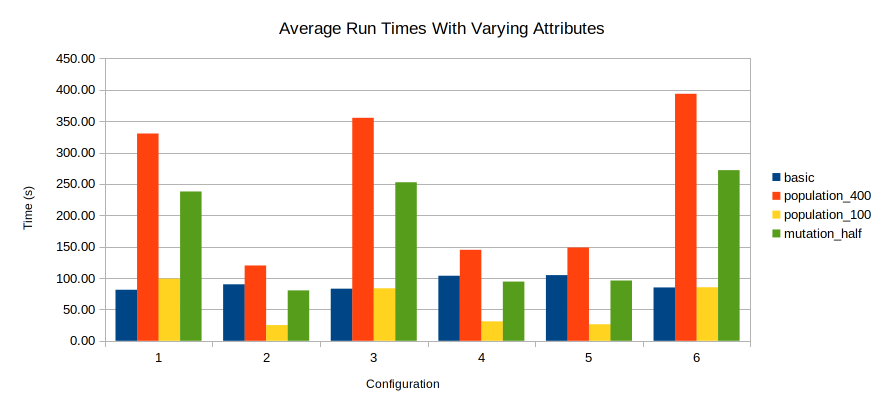
\includegraphics[width=1.0\textwidth]{images/inst-13-run-time.png}
\caption{\label{fig:inst-13-run-time}Average run time for inst-13.tsp file versus required configurations}
\end{figure}

In figure \ref{fig:inst-13-run-time} the results again are as expected. Increasing the population size obviously increases the runtime. It is worth noting that this file took significantly longer than inst-0.tsp and inst-16.tsp to process. Most likely this is down to this file being the largest dataset of the three.

\begin{figure}[H]
\vspace{-5pt}
\centering
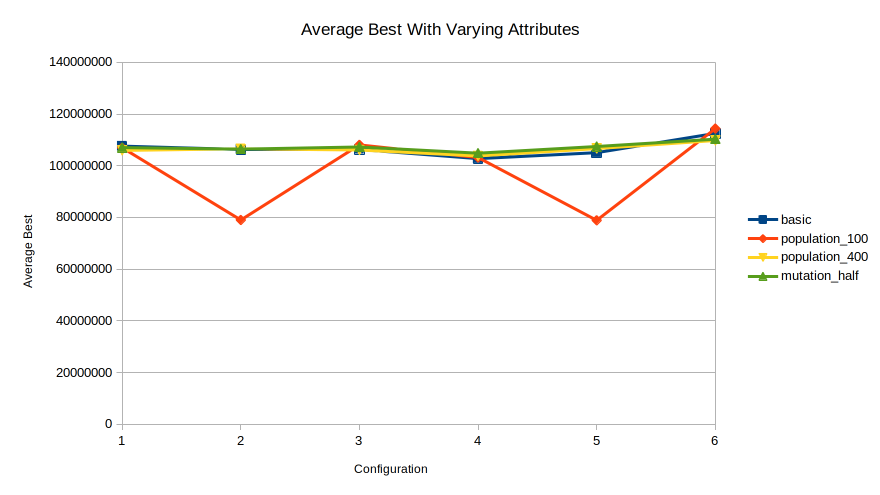
\includegraphics[width=1.0\textwidth]{images/inst-13-average-best.png}
\caption{\label{fig:inst-13-average-best}Average best results for inst-13.tsp file versus required configurations}
\end{figure}

Figure \ref{fig:inst-13-average-best} shows the average best results. This graph is more interesting than the inst-0.tsp results in that all of the variations except increasing the population size are similar across all configurations. Increasing the population size shows better results in configurations 2 and 5. 

\begin{figure}[H]
\vspace{-5pt}
\centering
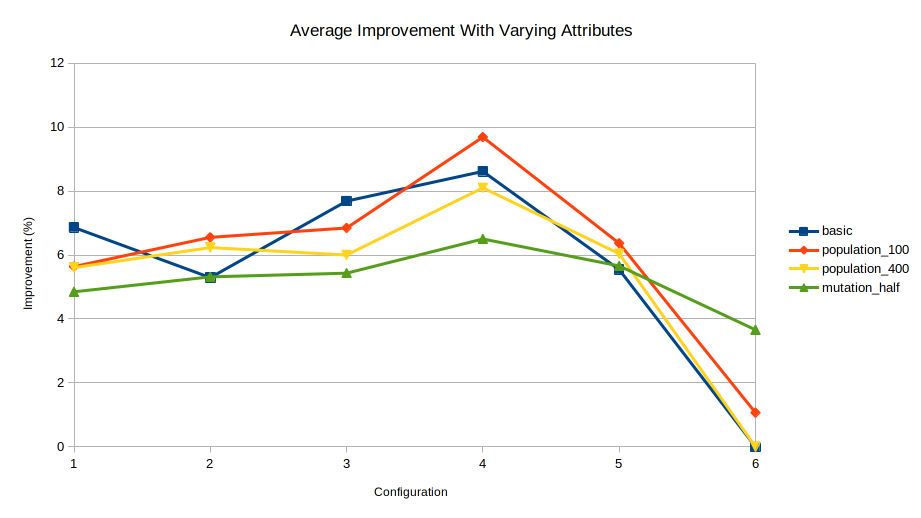
\includegraphics[width=1.0\textwidth]{images/inst-13-best-improvements.png}
\caption{\label{fig:inst-13-best-improvements}Average best improvements for inst-13.tsp file versus required configurations}
\end{figure}

\subsection{Results for inst-16.tsp}

For \textit{inst-16.tsp} file the below results have been collected with varying attributes.

\begin{itemize}
  \item Population size of 300
  \item Mutation rate of 0.1
  \item Max iterations of 300
\end{itemize}

\begin{table}[H]
\resizebox{\textwidth}{!}{%
\begin{tabular}{lllllll}
\rowcolor[HTML]{ECF4FF} 
Configuration                               & 1                  & 2                & 3                & 4                & 5                & 6                \\
\cellcolor[HTML]{ECF4FF}Time (s)            & 63                 & 79               & 65               & 91               & 93               & 68               \\
\cellcolor[HTML]{ECF4FF}Initial Best        & 110707719.099458   & 109336519.047216 & 113396253.510025 & 108927804.945994 & 103703934.993503 & 106714623.987208 \\
\cellcolor[HTML]{ECF4FF}Best                & 104256255.681925   & 102293954.842151 & 101547908.60348  & 100382657.076721 & 102767607.174564 & 106714623.987208 \\
\cellcolor[HTML]{ECF4FF}Improvement (\%)    & 5.83               & 6.44             & 10.45            & 7.84             & 0.90             & 0.00             \\
\cellcolor[HTML]{ECF4FF}                    &                    &                  &                  &                  &                  &                  \\
\cellcolor[HTML]{ECF4FF}Time (s)            & 63                 & 78               & 65               & 90               & 93               & 67               \\
\cellcolor[HTML]{ECF4FF}Initial Best        & 112145595.758945   & 109501014.323574 & 112008047.085283 & 109259441.200283 & 111743208.456674 & 111218483.887683 \\
\cellcolor[HTML]{ECF4FF}Best                & 104070505.739842   & 100336582.872797 & 104955543.124328 & 99609913.0148023 & 102255759.970133 & 105335448.237844 \\
\cellcolor[HTML]{ECF4FF}Improvement (\%)    & 7.20               & 8.37             & 6.30             & 8.83             & 8.49             & 5.29             \\
\cellcolor[HTML]{ECF4FF}                    &                    &                  &                  &                  &                  &                  \\
\cellcolor[HTML]{ECF4FF}Time (s)            & 64                 & 78               & 65               & 92               & 93               & 67               \\
\cellcolor[HTML]{ECF4FF}Initial Best        & 109429259.115128   & 111004234.510093 & 110778313.91191  & 110106041.232521 & 107987959.877032 & 110330563.40469  \\
\cellcolor[HTML]{ECF4FF}Best                & 103979638.15903191 & 101366595.356286 & 102605978.515632 & 100605341.928382 & 103299909.271958 & 108912194.665422 \\
\cellcolor[HTML]{ECF4FF}Improvement(\%)     & 4.98               & 8.68             & 7.38             & 8.63             & 4.34             & 1.29             \\
\rowcolor[HTML]{CBCEFB} 
\cellcolor[HTML]{DAE8FC}Average Run Time    & 63.33              & 78.33            & 65.00            & 91.00            & 93.00            & 67.33            \\
\rowcolor[HTML]{CBCEFB} 
\cellcolor[HTML]{DAE8FC}Average Best        & 104163380.710884   & 101332377.690411 & 103036476.747813 & 100199304.006635 & 102774425.472218 & 106987422.296825 \\
\rowcolor[HTML]{CBCEFB} 
\cellcolor[HTML]{DAE8FC}Average Improvement & 6.00               & 7.83             & 8.04             & 8.44             & 4.58             & 2.19             \\
\rowcolor[HTML]{CBCEFB} 
\cellcolor[HTML]{DAE8FC}Median              & 104163380.710884   & 101366595.356286 & 102605978.515632 & 100382657.076721 & 102767607.174564 & 106714623.987208
\end{tabular}%
}
\end{table}

\begin{itemize}
  \item Population size of 400
  \item Mutation rate of 0.1
  \item Max iterations of 300
\end{itemize}

\begin{table}[H]
\resizebox{\textwidth}{!}{%
\begin{tabular}{lllllll}
\rowcolor[HTML]{ECF4FF} 
Configuration                               & 1                & 2                & 3                & 4                & 5                & 6                \\
\cellcolor[HTML]{ECF4FF}Time (s)            & 259              & 106              & 287              & 128              & 132              & 336              \\
\cellcolor[HTML]{ECF4FF}Initial Best        & 109919499.628167 & 109863122.034262 & 109645941.762519 & 110827528.084609 & 107173744.44915  & 109437945.216138 \\
\cellcolor[HTML]{ECF4FF}Best                & 100697007.464198 & 102197984.608335 & 102116139.661403 & 98586661.9458835 & 103551479.697608 & 109437945.216138 \\
\cellcolor[HTML]{ECF4FF}Improvement (\%)    & 8.39             & 6.98             & 6.87             & 11.04            & 3.38             & 0.00             \\
\cellcolor[HTML]{ECF4FF}                    &                  &                  &                  &                  &                  &                  \\
\cellcolor[HTML]{ECF4FF}Time (s)            & 257              & 106              & 284              & 128              & 133              & 345              \\
\cellcolor[HTML]{ECF4FF}Initial Best        & 110257692.641786 & 110441235.33334  & 109374210.72773  & 109478142.582255 & 109098528.441088 & 109574146.101933 \\
\cellcolor[HTML]{ECF4FF}Best                & 100279340.719392 & 103020735.97998  & 102705489.604411 & 95347503.0994922 & 98750001.8862013 & 109574146.101933 \\
\cellcolor[HTML]{ECF4FF}Improvement (\%)    & 9.05             & 6.72             & 6.10             & 12.91            & 9.49             & 0.00             \\
\cellcolor[HTML]{ECF4FF}                    &                  &                  &                  &                  &                  &                  \\
\cellcolor[HTML]{ECF4FF}Time (s)            & 259              & 105              & 284              & 129              & 133              & 327              \\
\cellcolor[HTML]{ECF4FF}Initial Best        & 108025969.294326 & 109451822.4022   & 107321324.51066  & 108783843.973276 & 109187298.301254 & 108863427.797359 \\
\cellcolor[HTML]{ECF4FF}Best                & 104016437.512322 & 100443745.071925 & 103266110.44544  & 96121822.7330776 & 100031240.916388 & 108863427.797359 \\
\cellcolor[HTML]{ECF4FF}Improvement(\%)     & 3.71             & 8.23             & 3.78             & 11.64            & 8.39             & 0.00             \\
\rowcolor[HTML]{CBCEFB} 
\cellcolor[HTML]{DAE8FC}Average Run Time    & 258.33           & 105.67           & 285.00           & 128.33           & 132.67           & 336.00           \\
\rowcolor[HTML]{CBCEFB} 
\cellcolor[HTML]{DAE8FC}Average Best        & 101664261.898637 & 101887488.553413 & 102695913.237085 & 96685329.2594844 & 100777574.166732 & 109291839.705143 \\
\rowcolor[HTML]{CBCEFB} 
\cellcolor[HTML]{DAE8FC}Average Improvement & 7.05             & 7.31             & 5.58             & 11.86            & 7.08             & 0.00             \\
\rowcolor[HTML]{CBCEFB} 
\cellcolor[HTML]{DAE8FC}Median              & 100697007.464198 & 102197984.608335 & 102705489.604411 & 96121822.7330776 & 100031240.916388 & 109437945.216138
\end{tabular}%
}
\end{table}

\begin{itemize}
  \item Population size of 100
  \item Mutation rate of 0.1
  \item Max iterations of 300
\end{itemize}

\begin{table}[H]
\resizebox{\textwidth}{!}{%
\begin{tabular}{lllllll}
\rowcolor[HTML]{ECF4FF} 
Configuration                               & 1                & 2                & 3                & 4                & 5                & 6                \\
\cellcolor[HTML]{ECF4FF}Time (s)            & 64               & 25               & 66               & 27               & 28               & 68               \\
\cellcolor[HTML]{ECF4FF}Initial Best        & 111529237.597618 & 113903391.692222 & 113678463.577162 & 110974617.248596 & 111320563.130241 & 110550945.980378 \\
\cellcolor[HTML]{ECF4FF}Best                & 105753281.583507 & 101924283.995421 & 104007012.60592  & 97481168.7557805 & 105721416.369345 & 110550945.980378 \\
\cellcolor[HTML]{ECF4FF}Improvement (\%)    & 5.18             & 10.52            & 8.51             & 12.16            & 5.03             & 0.00             \\
\cellcolor[HTML]{ECF4FF}                    &                  &                  &                  &                  &                  &                  \\
\cellcolor[HTML]{ECF4FF}Time (s)            & 63               & 26               & 65               & 27               & 27               & 67               \\
\cellcolor[HTML]{ECF4FF}Initial Best        & 108829295.140042 & 110387269.712681 & 111397867.967366 & 113758040.466151 & 107031961.945045 & 114022501.464114 \\
\cellcolor[HTML]{ECF4FF}Best                & 102044172.593024 & 103576851.730826 & 103628442.136203 & 102026940.410423 & 103661014.716388 & 108809646.571734 \\
\cellcolor[HTML]{ECF4FF}Improvement (\%)    & 6.23             & 6.17             & 6.97             & 10.31            & 3.15             & 4.57             \\
\cellcolor[HTML]{ECF4FF}                    &                  &                  &                  &                  &                  &                  \\
\cellcolor[HTML]{ECF4FF}Time (s)            & 64               & 25               & 65               & 27               & 27               & 68               \\
\cellcolor[HTML]{ECF4FF}Initial Best        & 110749614.154982 & 111560088.321369 & 109977698.007253 & 111694677.534919 & 109038727.107981 & 111902796.009472 \\
\cellcolor[HTML]{ECF4FF}Best                & 103998092.349012 & 103656582.730221 & 104507115.440151 & 101568937.471364 & 104017745.816019 & 109993572.954042 \\
\cellcolor[HTML]{ECF4FF}Improvement(\%)     & 6.10             & 7.08             & 4.97             & 9.07             & 4.60             & 1.71             \\
\rowcolor[HTML]{CBCEFB} 
\cellcolor[HTML]{DAE8FC}Average Run Time    & 63.67            & 25.33            & 65.33            & 27.00            & 27.33            & 67.67            \\
\rowcolor[HTML]{CBCEFB} 
\cellcolor[HTML]{DAE8FC}Average Best        & 103931848.841848 & 103052572.818823 & 104047523.394091 & 100359015.545856 & 104466725.633917 & 109784721.835385 \\
\rowcolor[HTML]{CBCEFB} 
\cellcolor[HTML]{DAE8FC}Average Improvement & 5.84             & 7.92             & 6.82             & 10.51            & 4.26             & 2.09             \\
\rowcolor[HTML]{CBCEFB} 
\cellcolor[HTML]{DAE8FC}Median              & 103998092.349012 & 103576851.730826 & 104007012.60592  & 101568937.471364 & 104017745.816019 & 109993572.954042
\end{tabular}%
}
\end{table}

\begin{itemize}
  \item Population size of 300
  \item Mutation rate of 0.5
  \item Max iterations of 300
\end{itemize}

\begin{table}[H]
\resizebox{\textwidth}{!}{%
\begin{tabular}{lllllll}
\rowcolor[HTML]{ECF4FF} 
Configuration                               & 1                & 2                & 3                & 4                & 5                & 6                \\
\cellcolor[HTML]{ECF4FF}Time (s)            & 184              & 71               & 200              & 84               & 92               & 219              \\
\cellcolor[HTML]{ECF4FF}Initial Best        & 108798884.632561 & 106583464.472165 & 110456689.58687  & 109613270.505956 & 110078812.805607 & 111609370.841863 \\
\cellcolor[HTML]{ECF4FF}Best                & 103718148.940862 & 101608477.338846 & 101132840.373201 & 101643071.662153 & 103023056.16373  & 110343530.046084 \\
\cellcolor[HTML]{ECF4FF}Improvement (\%)    & 4.67             & 4.67             & 8.44             & 7.27             & 6.41             & 1.13             \\
\cellcolor[HTML]{ECF4FF}                    &                  &                  &                  &                  &                  &                  \\
\cellcolor[HTML]{ECF4FF}Time (s)            & 183              & 75               & 200              & 85               & 90               & 221              \\
\cellcolor[HTML]{ECF4FF}Initial Best        & 109036207.474106 & 108308497.784376 & 107816236.507507 & 107003511.864774 & 104560427.908373 & 105537211.290208 \\
\cellcolor[HTML]{ECF4FF}Best                & 102018780.818315 & 104392487.275674 & 101649100.720432 & 98673243.8255933 & 102008917.636734 & 105537211.290208 \\
\cellcolor[HTML]{ECF4FF}Improvement (\%)    & 6.44             & 3.62             & 5.72             & 7.79             & 2.44             & 0.00             \\
\cellcolor[HTML]{ECF4FF}                    &                  &                  &                  &                  &                  &                  \\
\cellcolor[HTML]{ECF4FF}Time (s)            & 184              & 73               & 199              & 87               & 88               & 218              \\
\cellcolor[HTML]{ECF4FF}Initial Best        & 108815036.127086 & 109111143.038363 & 110281840.590277 & 111456487.103784 & 110225134.390687 & 111530999.209681 \\
\cellcolor[HTML]{ECF4FF}Best                & 102897783.645376 & 101345754.289198 & 102880394.684506 & 100790957.527907 & 104494259.55014  & 111530999.209681 \\
\cellcolor[HTML]{ECF4FF}Improvement(\%)     & 5.44             & 7.12             & 6.71             & 9.57             & 5.20             & 0.00             \\
\rowcolor[HTML]{CBCEFB} 
\cellcolor[HTML]{DAE8FC}Average Run Time    & 183.67           & 73.00            & 199.67           & 85.33            & 90.00            & 219.33           \\
\rowcolor[HTML]{CBCEFB} 
\cellcolor[HTML]{DAE8FC}Average Best        & 102878237.801518 & 102448906.301239 & 101887445.25938  & 100369091.005218 & 103175411.116868 & 109137246.848658 \\
\rowcolor[HTML]{CBCEFB} 
\cellcolor[HTML]{DAE8FC}Average Improvement & 5.51             & 5.13             & 6.96             & 8.21             & 4.68             & 0.38             \\
\rowcolor[HTML]{CBCEFB} 
\cellcolor[HTML]{DAE8FC}Median              & 102897783.645376 & 101608477.338846 & 101649100.720432 & 100790957.527907 & 103023056.16373  & 110343530.046084
\end{tabular}%
}
\end{table}

\begin{figure}[H]
\vspace{-5pt}
\centering
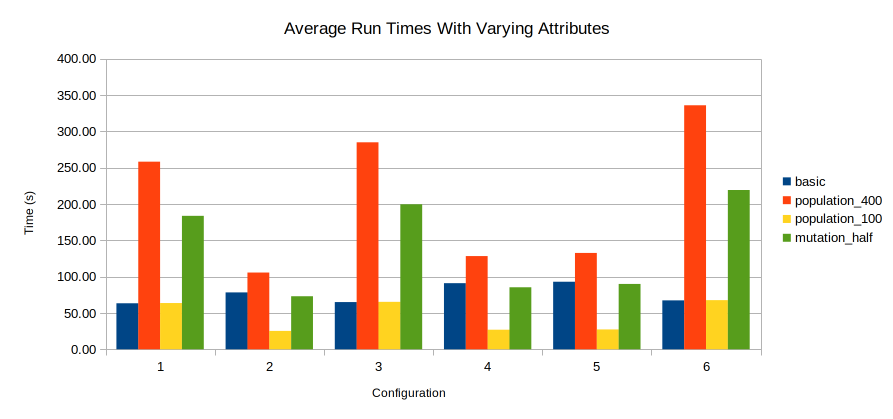
\includegraphics[width=1.0\textwidth]{images/inst-16run-time.png}
\caption{\label{fig:inst-16-run-time}Average run time for inst-16.tsp file versus required configurations}
\end{figure}

As can be seen from the results in \ref{fig:inst-16-run-time} this file was the second largest file of the three and the run times are in between inst-0.tsp and inst-13.tsp.

\begin{figure}[H]
\vspace{-5pt}
\centering
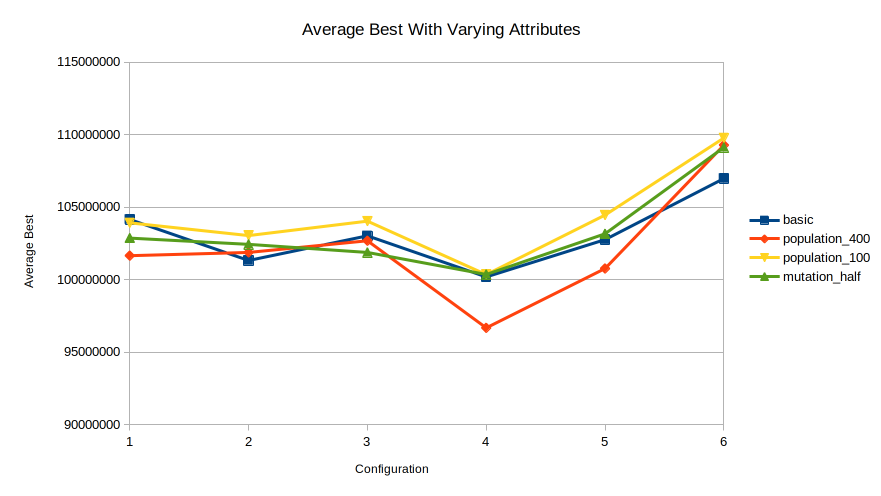
\includegraphics[width=1.0\textwidth]{images/inst-16-average-best.png}
\caption{\label{fig:inst-16-average-best}Average best results for inst-16.tsp file versus required configurations}
\end{figure}

\begin{figure}[H]
\vspace{-5pt}
\centering
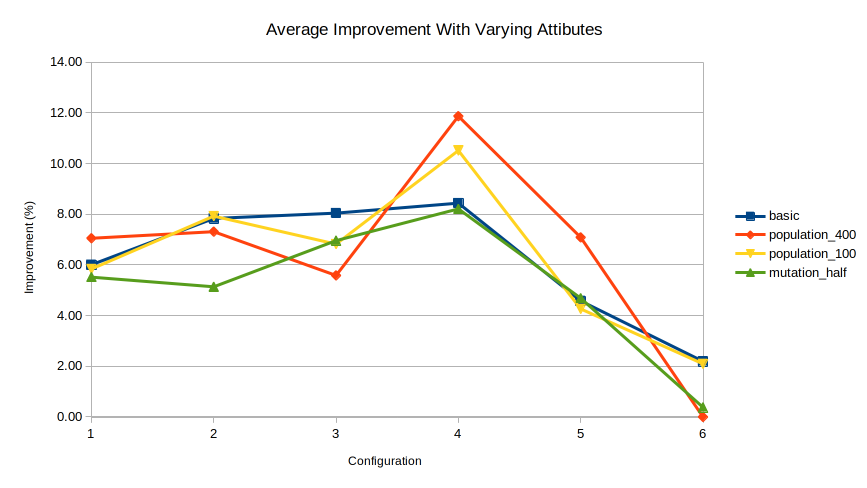
\includegraphics[width=1.0\textwidth]{images/inst-16-best-improvements.png}
\caption{\label{fig:inst-16-best-improvements}Average best improvements for inst-16.tsp file versus required configurations}
\end{figure}

\section{Summary}

The final conclusion for the best and worst operators is outlined in the table below

\begin{table}[H]
\resizebox{\textwidth}{!}{%
\begin{tabular}{
>{\columncolor[HTML]{ECF4FF}}l lll}
                    & \cellcolor[HTML]{ECF4FF}inst-0.tsp                                                                                                            & \cellcolor[HTML]{ECF4FF}inst-13.tsp                                                                                                                 & \cellcolor[HTML]{ECF4FF}inst-16.tsp                                                                                                                 \\
Best Configuration  & \begin{tabular}[c]{@{}l@{}}Increasing mutation to 0.5\\ Configuration 2\\ Random selection\\ Cycle crossover\\ Scramble mutation\end{tabular} & \begin{tabular}[c]{@{}l@{}}Decrease population to 100\\ Configuration 5\\ Roulette wheel\\ Uniform crossover\\ Scramble mutation\end{tabular}       & \begin{tabular}[c]{@{}l@{}}Increase population to 400\\ Configuration 4\\ Roulette wheel\\ Cycle crossover\\ Reciprocal exchange\end{tabular}       \\
Worst Configuration & \begin{tabular}[c]{@{}l@{}}Basic setup\\ Configuration 6\\ Best and second best\\ Uniform crossover\\ Scramble mutation\end{tabular}          & \begin{tabular}[c]{@{}l@{}}Decrease population to 100\\ Configuration 6\\ Best and second best\\ Uniform crossover\\ Scramble mutation\end{tabular} & \begin{tabular}[c]{@{}l@{}}Increasing mutation to 0.5\\ Configuration 6\\ Best and second best\\ Uniform crossover\\ Scramble mutation\end{tabular} \\
Best result         & 21027147.65                                                                                                                                   & 21346365.09                                                                                                                                         & 95347503.1                                                                                                                                          \\
Worst result        & 23001623.90                                                                                                                                   & 115089243.1                                                                                                                                         & 111530999.21                                                                                                                                       
\end{tabular}%
}
\end{table}